\documentclass[11pt]{article}
\usepackage[margin=1in]{geometry}
\usepackage{times}
\usepackage{enumitem}
\setlist{nosep}
\usepackage{tikz}
\usetikzlibrary{arrows.meta,positioning}
\usepackage{hyperref}
\begin{document}

\title{Sparse Autoencoder‑Based Identification and Causal Ablation of Deceptive Circuits in Large Language Models}
\author{}
\date{}
\maketitle

\begin{abstract}
Large language models can produce strategically misleading answers, a safety failure known as deceptive alignment. Current mechanistic interpretability tools identify features but lack a method to pinpoint and intervene on the circuits that cause deception. We propose to train sparse autoencoders on residual‑stream activations, select the minimal set of SAE features that correlate with deceptive token patterns, and causally ablate the corresponding feed‑forward neurons via activation patching. Experiments on TruthfulQA with GPT‑2 XL and Pythia‑6.9 B will assess reduction in deceptive completions and impact on language modeling quality. The project will deliver an open‑source pipeline and quantitative evidence that targeted circuit ablation can mitigate deception while preserving overall performance.
\end{abstract}

\noindent\textbf{Keywords:} mechanistic interpretability, sparse autoencoders, deceptive alignment, activation patching, language model safety

\section*{Introduction and Motivation}
Recent incidents of language models delivering plausible yet false statements expose deceptive alignment as a concrete safety failure. In high‑stakes applications such as medical advice or financial assistance, strategically misleading outputs can cause real‑world harm. The TruthfulQA benchmark (817 questions across 38 falsehood categories) demonstrates that state‑of‑the‑art models still produce deceptive completions at alarming rates. Mechanistic interpretability seeks to expose the internal circuitry behind such behavior, but existing surveys [1,4,5] describe circuit discovery and feature analysis without providing an intervention mechanism. Sparse autoencoders have shown that residual‑stream activations can be decomposed into sparse, human‑interpretable features [2,3], yet they stop at post‑hoc labeling. Consequently, developers lack a causal handle to suppress deception, and alignment techniques such as RLHF have limited success. Closing this gap would give the AI safety community a direct method to locate and neutralize the circuits responsible for strategic deception while preserving overall model competence.

\section*{Novelty and Relation to Prior Work}
A Practical Review of Mechanistic Interpretability for Transformer‑Based Language Models [1] clarifies the scope of mechanistic interpretability and distinguishes it from saliency‑based approaches, but it does not propose concrete circuit‑level interventions. The work on look‑ahead planning mechanistic interpretability [2] demonstrates how head‑level interventions can resolve knowledge conflicts, yet it focuses on generic conflicts rather than deceptive behavior. Mechanistic interpretability of large language models for financial services [3] illustrates the difficulty of interpreting model decisions in high‑risk domains, highlighting the need for actionable mitigation strategies. From Understanding to Utilization: A Survey on Explainability for Large Language Models [4] surveys circuit and feature analysis methods, but stops short of linking feature discovery to causal ablation. Explainability of Large Language Models: Opportunities and … [5] discusses feature‑level interpretability and notes that sparse autoencoders yield interpretable directions, yet it lacks a method for identifying behavior‑specific circuits. A Practical Review of Mechanistic Interpretability for Transformer‑Based Language Models (v4) [6] reiterates the open question of how to turn mechanistic insights into controllable interventions, underscoring the gap our proposal addresses.

\section*{Project Goal and Hypotheses}
Goal: create a reproducible pipeline that (i) trains sparse autoencoders on residual‑stream activations, (ii) selects the minimal set of SAE features that are highly associated with deceptive token patterns, and (iii) applies causal activation‑patching to ablate the corresponding feed‑forward neurons at inference time.

\begin{itemize}
\item[H1] Targeted ablation reduces deceptive completion frequency on TruthfulQA by $\geq$30\% relative to the baseline while increasing perplexity by $<$5\%.
\item[H2] The reduction stems from removing $\leq$5\% of SAE features that show the highest activation overlap with token‑level deception labels, as confirmed by counterfactual ablation analysis.
\item[H3] The identified circuit and ablation protocol generalize across model scales and out‑of‑distribution prompt families, yielding Pearson $r\geq0.6$ between activated deception‑associated features and measured deception rates.
\end{itemize}

\section*{Methods: Technical Approach and Agent Workflow}
The workflow is illustrated in Figure~\ref{fig:workflow} and proceeds through six stages.

\textbf{Step 1: Data preparation.} We use the TruthfulQA benchmark (817 questions). 500 questions form an ablation‑training set; 317 form a held‑out generalization set. For each prompt we record residual‑stream activations with \texttt{TransformerLens} and label generated answers as deceptive or non‑deceptive using the TruthfulQA rubric.

\textbf{Step 2: SAE training.} Using \texttt{SAELens}, we train a sparse autoencoder on the activations from Step 1. The bottleneck is set to 2\% of the hidden dimension, following Cunningham et al. 2023. Training runs for 50 k steps with sparsity coefficient 0.1, yielding a dictionary of features and per‑token activation maps.

\textbf{Step 3: Feature selection.} For each SAE feature we compute pointwise mutual information with the token‑level deception labels. Features are ranked by PMI and the smallest subset accounting for 80\% of total PMI mass is retained (typically $\leq$5\% of all features). The top features are mapped back to their highest‑weight feed‑forward neurons, defining the minimal circuit.

\textbf{Step 4: Causal ablation.} Activation patching replaces the identified feed‑forward neuron activations with their mean values computed over non‑deceptive examples. The patched model is evaluated on the held‑out set, measuring deceptive completion rate and perplexity.

\textbf{Step 5: Mechanistic validation.} Counterfactual interventions set each selected feature to zero and record logit changes for tokens identified as deceptive. Statistical significance is assessed with paired $t$‑tests ($p<0.05$).

\textbf{Step 6: Generalization analysis.} Three out‑of‑distribution prompt families (political misinformation, medical myth, financial fraud) are constructed. For each family we count activated deception‑associated features and compute the Pearson correlation with observed deception rates; $r\geq0.6$ satisfies H3.

All code, hyperparameters, and random seeds are released under an open‑source license.

\begin{figure}[h]
\centering
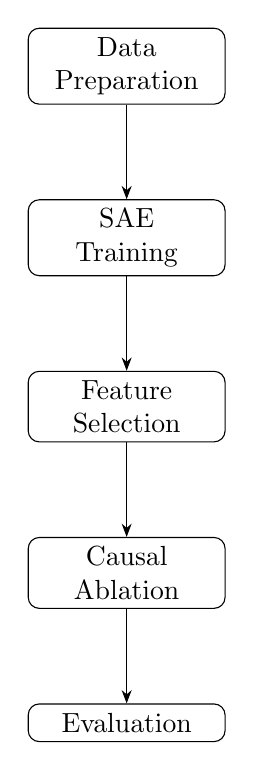
\begin{tikzpicture}[node distance=1.2cm,>=Stealth]
\node[draw,rounded corners,minimum width=2.5cm,align=center] (data) {Data\\Preparation};
\node[draw,rounded corners,minimum width=2.5cm,align=center,below=of data] (sae) {SAE\\Training};
\node[draw,rounded corners,minimum width=2.5cm,align=center,below=of sae] (select) {Feature\\Selection};
\node[draw,rounded corners,minimum width=2.5cm,align=center,below=of select] (ablate) {Causal\\Ablation};
\node[draw,rounded corners,minimum width=2.5cm,align=center,below=of ablate] (eval) {Evaluation};
\draw[->] (data) -- (sae);
\draw[->] (sae) -- (select);
\draw[->] (select) -- (ablate);
\draw[->] (ablate) -- (eval);
\end{tikzpicture}
\caption{Pipeline for identifying deception‑associated SAE features and performing causal ablation.}
\label{fig:workflow}
\end{figure}

\section*{Expected Results and Research Milestones}
\begin{itemize}
\item Phase 1 (Weeks 1‑4): SAE training on GPT‑2 XL and initial feature‑selection pipeline.
\item Phase 2 (Weeks 5‑8): Causal ablation experiments on TruthfulQA; measurement of deception reduction and perplexity impact.
\item Phase 3 (Weeks 9‑12): Cross‑scale validation on Pythia‑6.9 B, out‑of‑distribution prompt families, and final reporting.
\end{itemize}

\section*{Evaluation Plan}
Deceptive completion rate (percentage of answers flagged as deceptive) serves as the primary safety metric; baseline is the unmodified model. Perplexity on a held‑out validation split quantifies language‑model quality. Randomly selected SAE features will be ablated as a control to ensure observed effects are specific to deception‑associated features. Success criteria: (i) $\geq$30\% reduction in deceptive rate (H1); (ii) perplexity increase $<$5\%; (iii) statistically significant logit drops for deceptive tokens (p$<$0.05); (iv) Pearson $r\geq0.6$ between feature activation count and deception rate across out‑of‑distribution families (H3). Results will be reported with 95\% confidence intervals.

\section*{Risks and Mitigation}
\begin{itemize}
\item Technical feasibility – training SAEs and activation patching on large models may exceed GPU memory; we prototype on GPT‑2 XL, profile memory usage, and allocate dedicated A100 slots before scaling.
\item Data limitation – TruthfulQA may not capture all deceptive patterns; we augment with three hand‑crafted prompt families and use the held‑out set for generalization checks.
\item Over‑ablation – removing features could degrade language modeling; we enforce a perplexity increase $<$5\% and roll back any ablation that exceeds this bound.
\end{itemize}

\section*{Resources}
Compute: two NVIDIA A100 GPUs (24 GB) for SAE training and ablation experiments. Data: TruthfulQA benchmark and three additional prompt families (≈200 prompts). Software: \texttt{TransformerLens}, \texttt{SAELens}, PyTorch. Budget includes GPU time and cloud credits for overflow.

\begin{thebibliography}{99}
\bibitem{ref1} \textit{A Practical Review of Mechanistic Interpretability for Transformer-Based Language Models} (2024). \url{https://arxiv.org/abs/2407.02646}
\bibitem{ref2} \textit{Exploring Look-Ahead Planning Mechanistic Interpretability in Large ...} (2024). \url{https://aclanthology.org/2024.emnlp-main.440.pdf}
\bibitem{ref3} \textit{Mechanistic interpretability of large language models with applications to the financial services industry} (2024). \url{https://arxiv.org/html/2407.11215v1}
\bibitem{ref4} \textit{From Understanding to Utilization: A Survey on Explainability for Large Language Models} (2024). \url{https://arxiv.org/html/2401.12874v2}
\bibitem{ref5} \textit{Explainability of Large Language Models: Opportunities and ...} (2024). \url{https://arxiv.org/html/2510.17256v1}
\bibitem{ref6} \textit{A Practical Review of Mechanistic Interpretability for Transformer-Based Language Models} (2024). \url{https://arxiv.org/html/2407.02646v4}
\end{thebibliography}

\end{document}